\documentclass[dvisvgm]{standalone}

\usepackage{tikz}
\usetikzlibrary {arrows.meta, positioning, automata}

\begin{document}

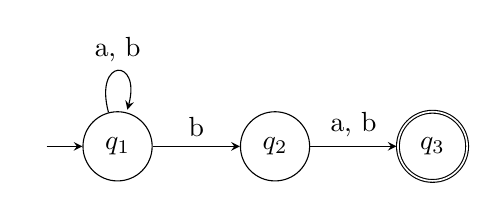
\begin{tikzpicture}[
    ->,
    >=stealth,
    node distance=2cm,
    initial text=$ $,
    on grid,
]

    \node[initial,   state]              (A) {$q_1$};
    \node[           state, right =of A] (B) {$q_2$};
    \node[accepting, state, right =of B] (C) {$q_3$};

    \path
        (A) edge [above]      node {b}     (B)
        (A) edge [loop above] node {a, b}  (A)
        (B) edge [above]      node {a, b}  (C)
    ;
\end{tikzpicture}

\end{document}